\chapter{Relevant Facts and Assumptions}

% facts and assumptions that are not constraints or requirements. E. g. intresting information, delining the context.
There are a wide variety of customers that Caruso is looking to acquire. \autoref{caruso-customers} shows which of them are the most valuable customers. Carvis should mainly focus on those in the top right corner, as they are the best prepared and represent the highest yield opportunity.

\begin{figure}[ht]
  \centering
  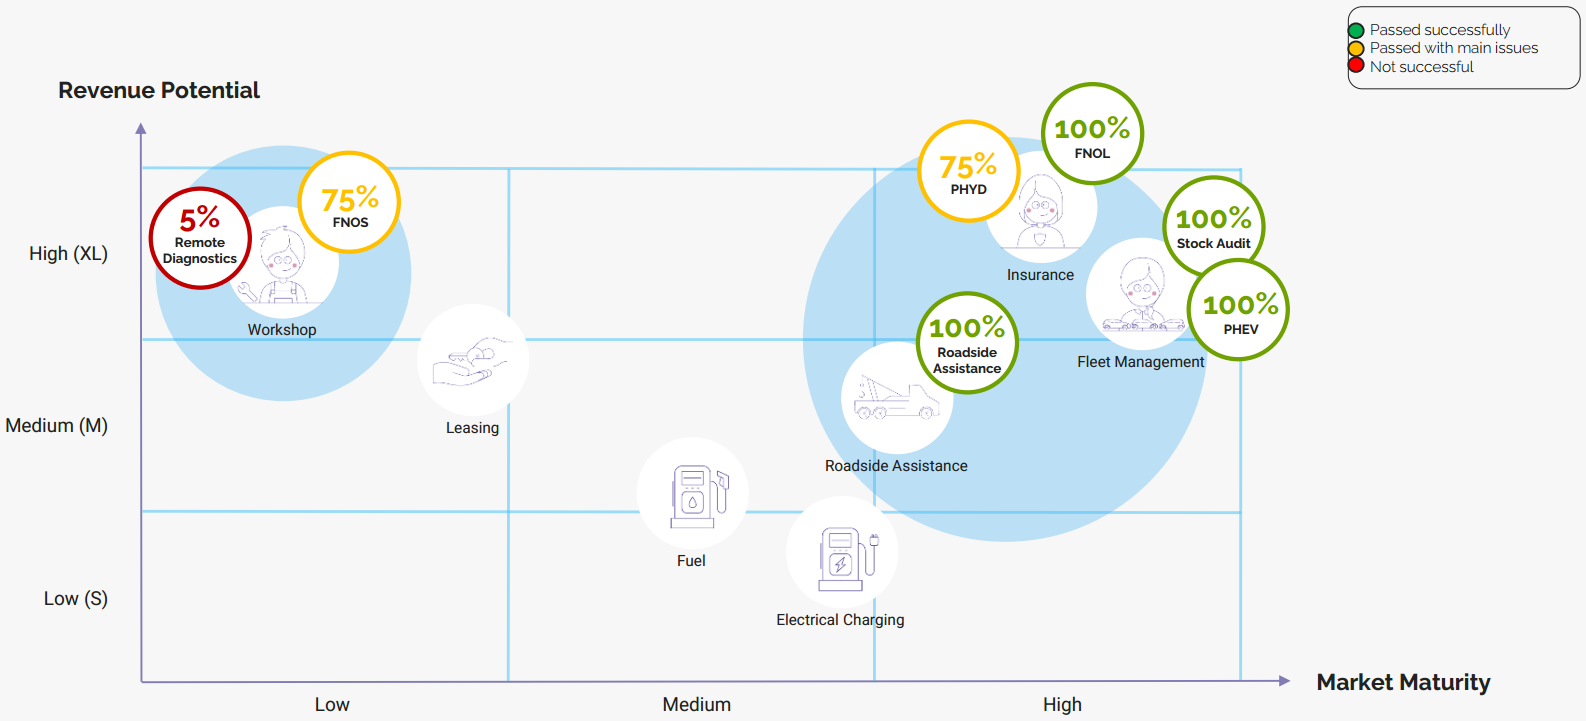
\includegraphics[width=\textwidth]{relevant_facts_and_assumptions/caruso-use-cases.png}
  \caption{Graph of different Caruso customers, they are ordered by revenue potential and market maturity.}
  \label{caruso-customers}
\end{figure}

A possible conclusion to the aforementioned statement could be that only large companies are compelling customers, which is not the case. Large companies have a lot of resources to invest in innovative technologies, so the demand for a data appetizer is lower. On the other hand mid-sized companies typically want to know what they are investing their money and time before allocating resources. This is where Carvis helps to highlight areas where Caruso data can be used.

Widgets designed as part of this project where not designed in cooperation with decision makers, instead the input of the Caruso sales employee was used. As a result of this, it is not certain that the widgets fit the needs of the specific use cases. The process of adjusting the widgets is the responsibility of the configurator. Talking to the decision makers is not part of the scope of this project.

The goal of this project is to deliver a finished product that meets the needs of our stakeholders, including Caruso. We understand that Caruso may not want to invest additional development time on their team to make adjustments to the application. As such, a modular system using widgets is the best solution for this project.